\documentclass[a4, oneside, 10pt, nobib]{memoir}
\usepackage{graphicx}
\usepackage{fontspec}
\usepackage{float}
	% Numbers={OldStyle,Proportional},Ligatures=TeX
	\setmainfont[]{Minion Pro}
	\setmonofont[Scale=0.85]{Iosevka}

\usepackage[backend=biber, style=numeric, defernumbers]{biblatex}
\addbibresource{bibliography.bib}
\setlrmarginsandblock{3.5cm}{2.5cm}{*}
\setulmarginsandblock{2.5cm}{*}{1}
\checkandfixthelayout 

\begin{document}
\thispagestyle{empty}

\begin{center}

	{\Large Antonio Vivace}
	\\
	\vspace{8mm}
	{\Huge \textbf{Modernising the CERN CMS Trigger Rates Monitoring software}}
	\\
	\vspace{8mm}
	{\huge Master Thesis Summary}
\end{center}

\pagebreak
\setcounter{page}{1}

		\paragraph{CERN, LHC and CMS} High Energy Physics experiments involve large amount of complex systems subject to anomalies and malfunctioning. They generate a lot of high dimensional data that must be monitored and analysed by various specialised teams to validate and deliver certified data for physics analysis. Most of these tasks are still carried out completely by humans, by looking at highly-contextual data and plots in complex workflows. Machine Learning techniques and approaches are being evaluated to aid and possibly automatize these processes.

		CERN, the European Organization for Nuclear Research, operates the Large Hadron Collider (LHC), the world's largest and highest-energy particle collider, one the largest machine in the world.

		2500 staff members design, construct and operate the research infrastructure, in addition to more than 17500 users and scientists of 110 nationalities, from institutes in more than 70 countries.

		The Compact Moun Solenoid (CMS) detector in the LHC is a complex system which needs fast and reliable monitoring. Quick feedback on each of the subsystems is essential to spot and solve problems or the data taken might be unusable or not interesting for physics analysis. Experts from different systems need to correlate information to investigate underlying problems.

\begin{figure}[H]
    \centerline{
        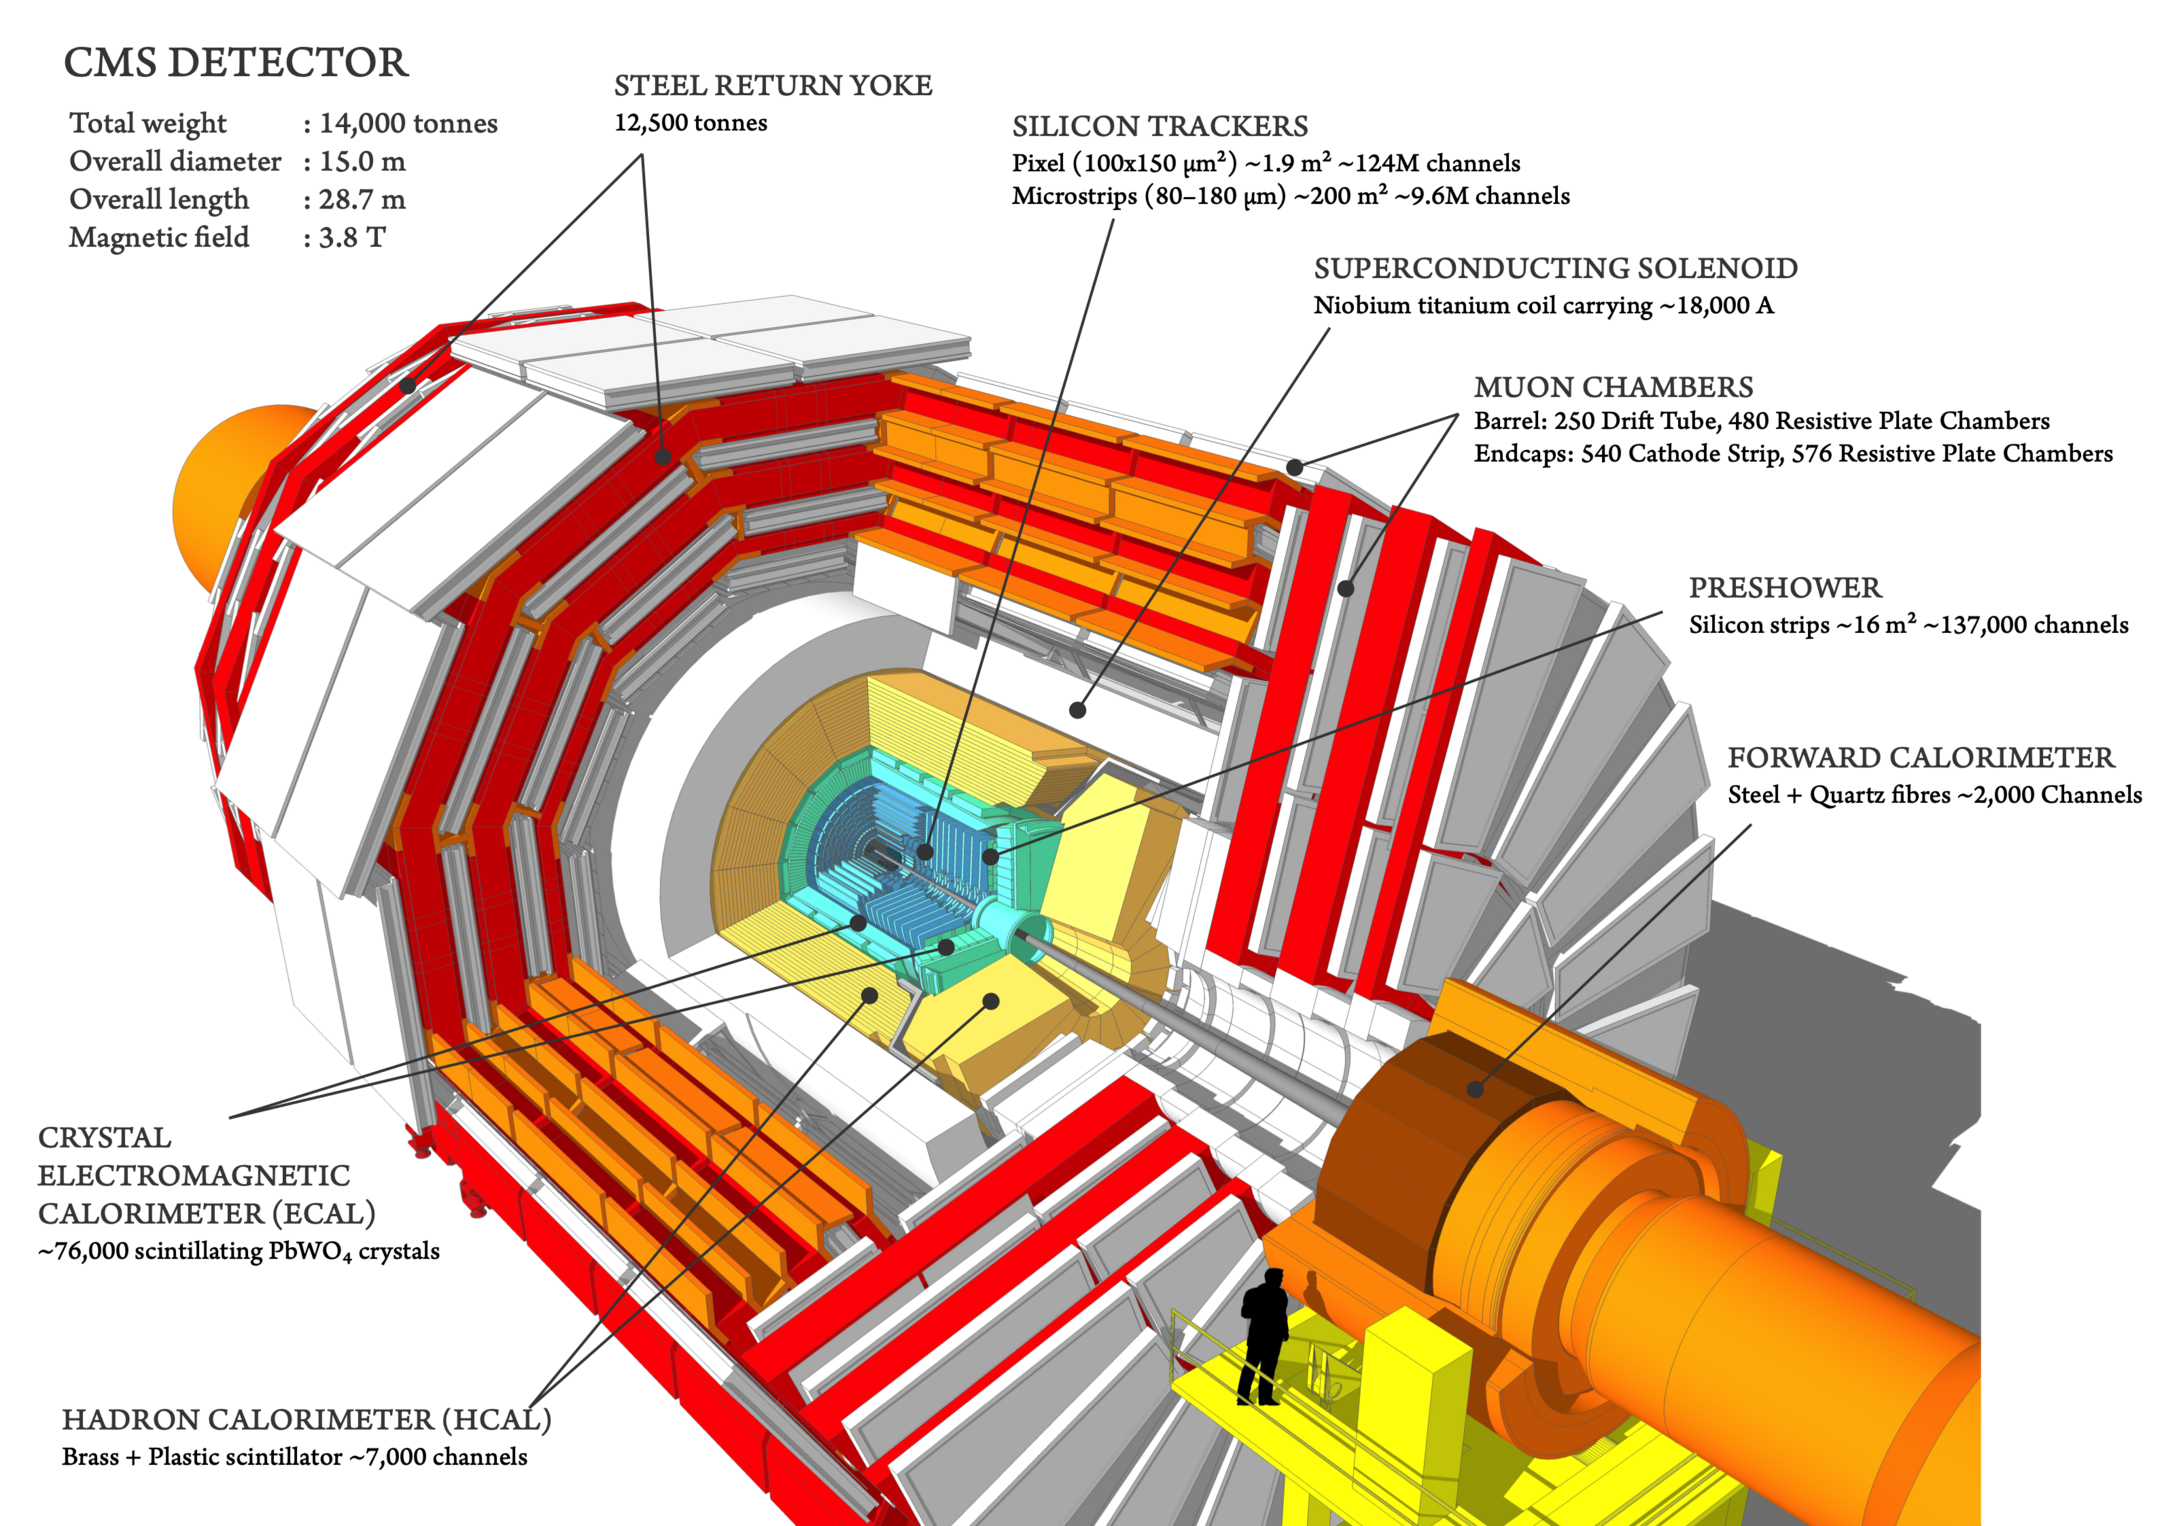
\includegraphics[width=0.8\paperwidth]{figures/cms}}
    \caption{Cutaway diagram of the CMS detector \cite{Sakuma_2014}}
    \label{fig:cms}
\end{figure}

		A centralized monitoring solution must expose real time data, historical information, summaries and reports from a series of heterogeneous sources. The Web Based Monitoring (WBM) software covered this role since the commissioning of the CMS experiment (2008), evolving and integrating new services into a growing framework during LHC Run 1 (2010-2013) and Run 2 (2015-2018).
\pagebreak
		\paragraph{Monitoring the Trigger System}

		A Trigger system is responsible of filtering the large majority of events, spotting the potentially interesting ones, triggering the detector's read-out system to retain data from the selected collisions.

		The CMS experiment generates milions of events per second, each one carrying payloads averaging \~{}1.5 MB \cite{smdaqatlhc2016v3pdf-2020-10-12}. One of the major challenges is the task of reducing event rate from roughly 40 MHz down to a more manageable 1 kHz while keeping as many interesting physics events as possible. This is accomplished through the use of a Level-1 (L1) \cite{Bayatyan:706847} hardware based trigger as well as a software based High-Level Trigger (HLT) \cite{Khachatryan_2017}. 



		This crucial phase is also sensible to malfunctions of many of the underlying parts, from sub detectors to the trigger algorithms configurations: monitoring the rates of such filters is essential to spot any anomalous behaviour in the underlying (sub)systems, software and/or hardware configurations, network and detector malfunctions.
		A trigger is a series or reconstruction steps and filters trying to select specific physics signatures like high momentum leptons or large energy deposits in the calorimeters \cite{TriggeringandDataAcquisitionCMSExperiment-2020-10-12}.



		Monitoring and understanding the output rates of the L1 and HLT triggers is of key importance for determining the overall performance of the trigger system and is intimately tied to what type of data is being recorded for physics analyses.


\begin{figure}[H]
    \centerline{
        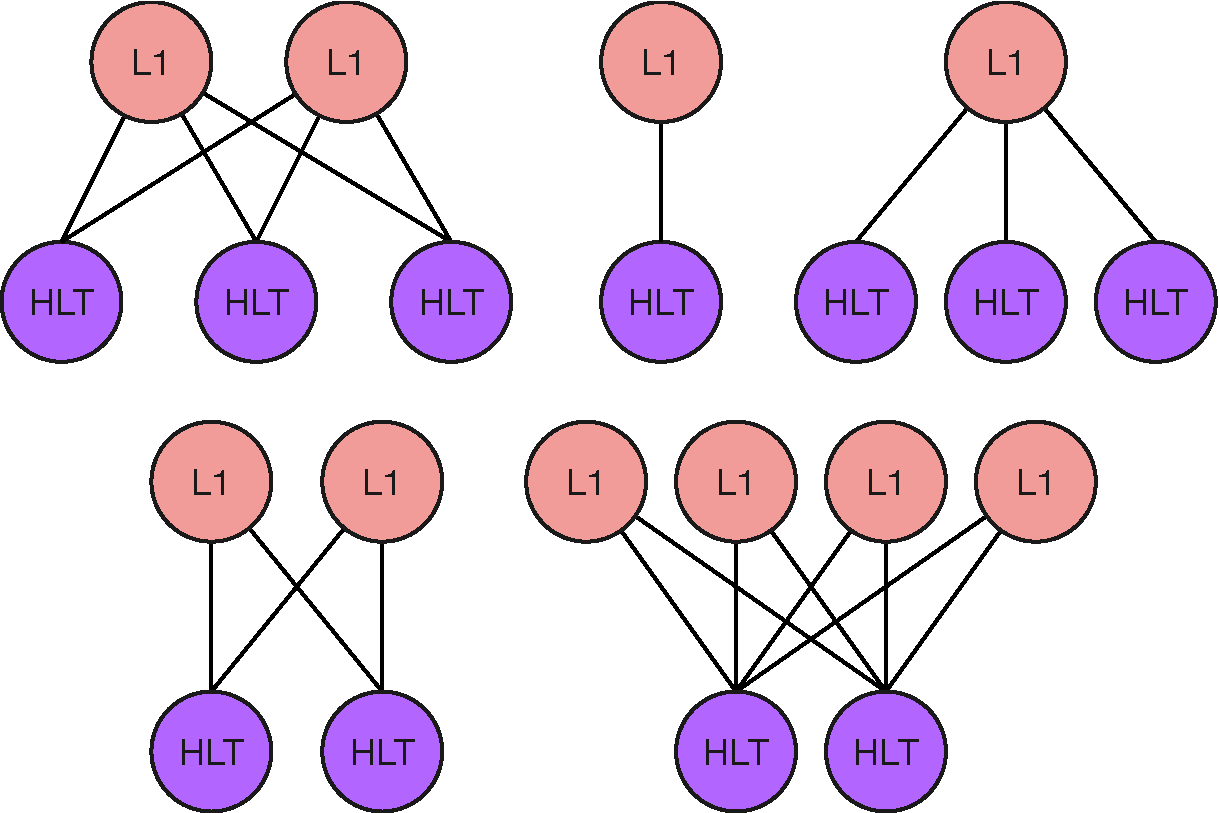
\includegraphics[width=0.35\paperwidth]{figures/triggers.pdf}}
    \caption{Simplified graph inspired by the trigger system configuration: the triggers connections can be seen as hierarchical directional graph. Red nodes represent L1 Trigger while purple HLT. Each link is directed from the red nodes to the purple ones. In reality, few hundred nodes spread approximately equally between HLT and L1 Trigger. \cite{adpol-cvae}}
    \label{fig:triggers}
\end{figure}



		This work concerns RateMon, the software framework providing the monitoring data on this Trigger system: it exposes Trigger Rates data, querying the OMDS database and carrying out \textbf{normalisations} and \textbf{corrections} for a number of different configurations and conditions, allowing consistent comparisons. It is powered by ROOT \cite{Brun:1997pa}, an open-source data analysis framework developed by CERN, and its Python interface, PyROOT.


		Trigger Rates are presented in the form of \textit{Rates VS PU} \textbf{plots}. It is also responsible of \textbf{alerting} the Trigger Shifters staff when rates deviate too much from the \textbf{predicted} values. Those predictions are based on analytical models fitted on data collected in previous runs.

		This software is also used by shifters in the CMS Control Room to monitor Trigger Rates and spot potential problems during the LHC runs.


		\paragraph{Upgrading the monitoring framework} 

		During the second Long Shutdown of the LHC (2018-2021) the CMS detector will be upgraded and many CMS sub-systems will drastically change. WBM started to show its age and problems: it unexpectedly and heavily grew with new features, arriving at a point where services were using vastly different technologies and it became harder and harder to mantain and expand. It has been decided to deprecate WBM in favor of a new software framework, called Online Monitoring System (OMS), decoupling the User Interface (UI) from the Aggregation (Data) Layer.

\begin{figure}[H]
    \centerline{
        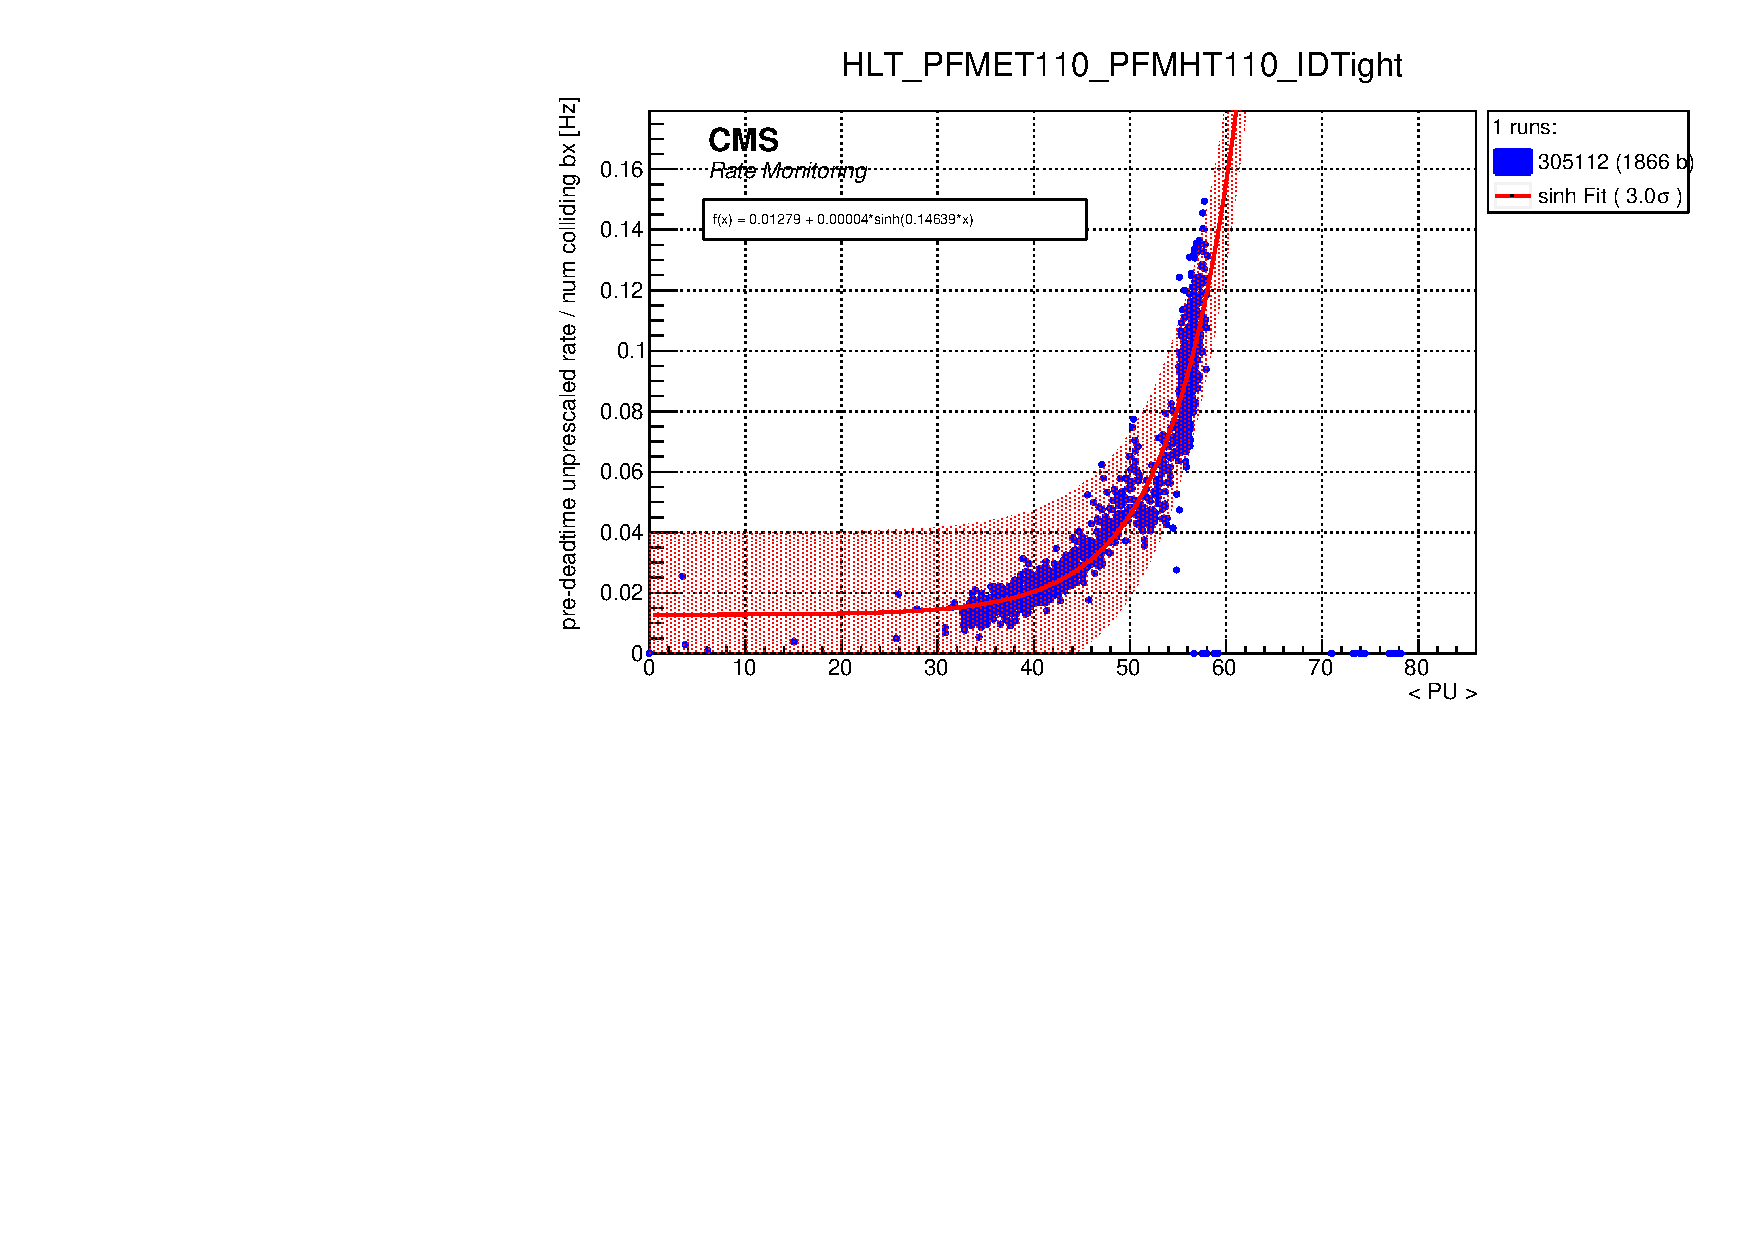
\includegraphics[width=0.6\paperwidth]{figures/RMT_305112_HLT_PFMET110_PFMHT110_IDTight.pdf}}
    \caption{An HLT Trigger path plotted with a fitted function on run 305112}
    \label{fig:ratemon_hlt}
\end{figure}


		\paragraph{Overview}

		We proceed to improve and renovate the set of tools included in RateMon, getting them ready to be migrated to the new OMS infrastructure: the tool can be now run and deployed in a reproducible and isolated way. A new CI/CD pipeline is implemented to streamline the development process and deliver software updated directly to the Control Room machines. A new API surface exposes the software analysis, model fitting and plotting capabilities.

		The following goals have been achieved and delivered in production \cite{VivaceRTM1} \cite{VivaceRTM2} \cite{L1TriggerOMSDevelopments} \cite{MohrmanRTM}:

		\begin{itemize}

		\item Upgraded the tools to run on a recent and supported version of Python and PyROOT.
		\item Moved the database connection configuration class to an configuration file.
		\item Formally defined the environment and the dependencies needed to run the software.
		\item To be compliant (and integrate) with control room deployment procedures, prepared scripts to package the software with the RPM package format. Prepared a basic systemd service to include in the package, to allow running the software as a system service.
		\item Prepared a Continuos Integration and Deployment pipeline running on the CERN infrastructure.
		\item Upgraded the CI/CD pipeline to use the CMS Cactus \cite{DirkxCactus} auto DevOps tools.
		\item Upgraded the exporting feature of the tools, previously limited to shell output and small PNG image renders.
		\item Enabled the tools to export trigger rates data in ROOT binary files, allowing ROOT clients to read them.
		\item Enabled the tools to export trigger rates data also in a agnostic format, not tied to ROOT.
		\item Updated the documentation adding a a way to consistently prepare any machine to run RateMon tools, without being tied to a particular machine cluster at CERN.
		\item Enabled any user to import the RateMon software as a Python module, adding some external-facing and transparent methods to get Trigger Rates as raw data or plots.
		\item Investigated a solution to integrate RateMon into the new CMS OMS, replacing the old Web Based Monitoring, now deprecated.
		\item Implemented an API exposing the exporting, processing and plotting functionalities of the RateMon software. This API is formally defined with an OpenAPI 3 Schema and an auto generated Swagger interface is available as documentation to users. This API can be plugged into the OMS stack to provide the old plots and many new features.
		\item Implemented a reactive web application in VueJS to demonstrate and showcase the API capabilities, plotting Trigger Rates (and their predicted values, based on the fits) in the browser with interactive and scalable plots (powered by JSROOT) instead of static image exports, consuming the new API.
		\item Implemented a Trigger Selection interface on the UI, a feature requested by Trigger shifters and coordinators.
		\item Reported a series of bugs happening in the data processing phase of the scripts, detailing scenarios triggering them, to allow future work on them.
		\item Deployed the implemented stack in production. Set up a separate data storage solution to cache computed data, limiting the bottleneck effect of the CMS database on the API and offering faster responses.

		\end{itemize}


		\paragraph{Building a new dataset to aid automated Anomaly Detection approaches}

		Trying to fit traditional Machine Learning (ML) pipelines and models in this task is not a novel idea: an elaborated research study has been conducted on Anomaly Detection and Machine Learning approaches to similar problems at CERN, from Variational Auto Encoders solutions \cite{adpol-cvae}aiming to improve the analytical models to fit and predict trigger rates to isolation forest and gaussian mixture models \cite{Halilovic:2665985} to detect anomalies in the LHC injection magnets.

		Similar papers and state of the art studies have been surveyed to frame and formally define our problem.

		Obtaining large, proportionally labeled datasets and the intrinsic difficulty to codify and formalise the human expertise in a "consumable" form for traditional ML pipelines appeared as the most critical points of these attemps.

		Therefore, we exploited the acquired knowledge on the software sources to produce a new integrated and labelled dataset.

		Additional work has been done to properly export data from another important source at CMS, the new Run Registry \cite{cms_collaboration_2019_3599323}. It exposes the status over time of every part of the detector, including the ones for which the failures are identifiable from the monitoring of the trigger rates, the process currently carried out by humans by looking at trigger plots, reference fits and other detector diagnostic data.

		These improvements enabled trigger rates time series and detector data to be properly exported and integrated in a new, rich dataset of genuine and labeled anomalous runs, possibily providing a new starting point for novel approaches to automatize this task.

\begin{figure}
    \centerline{
        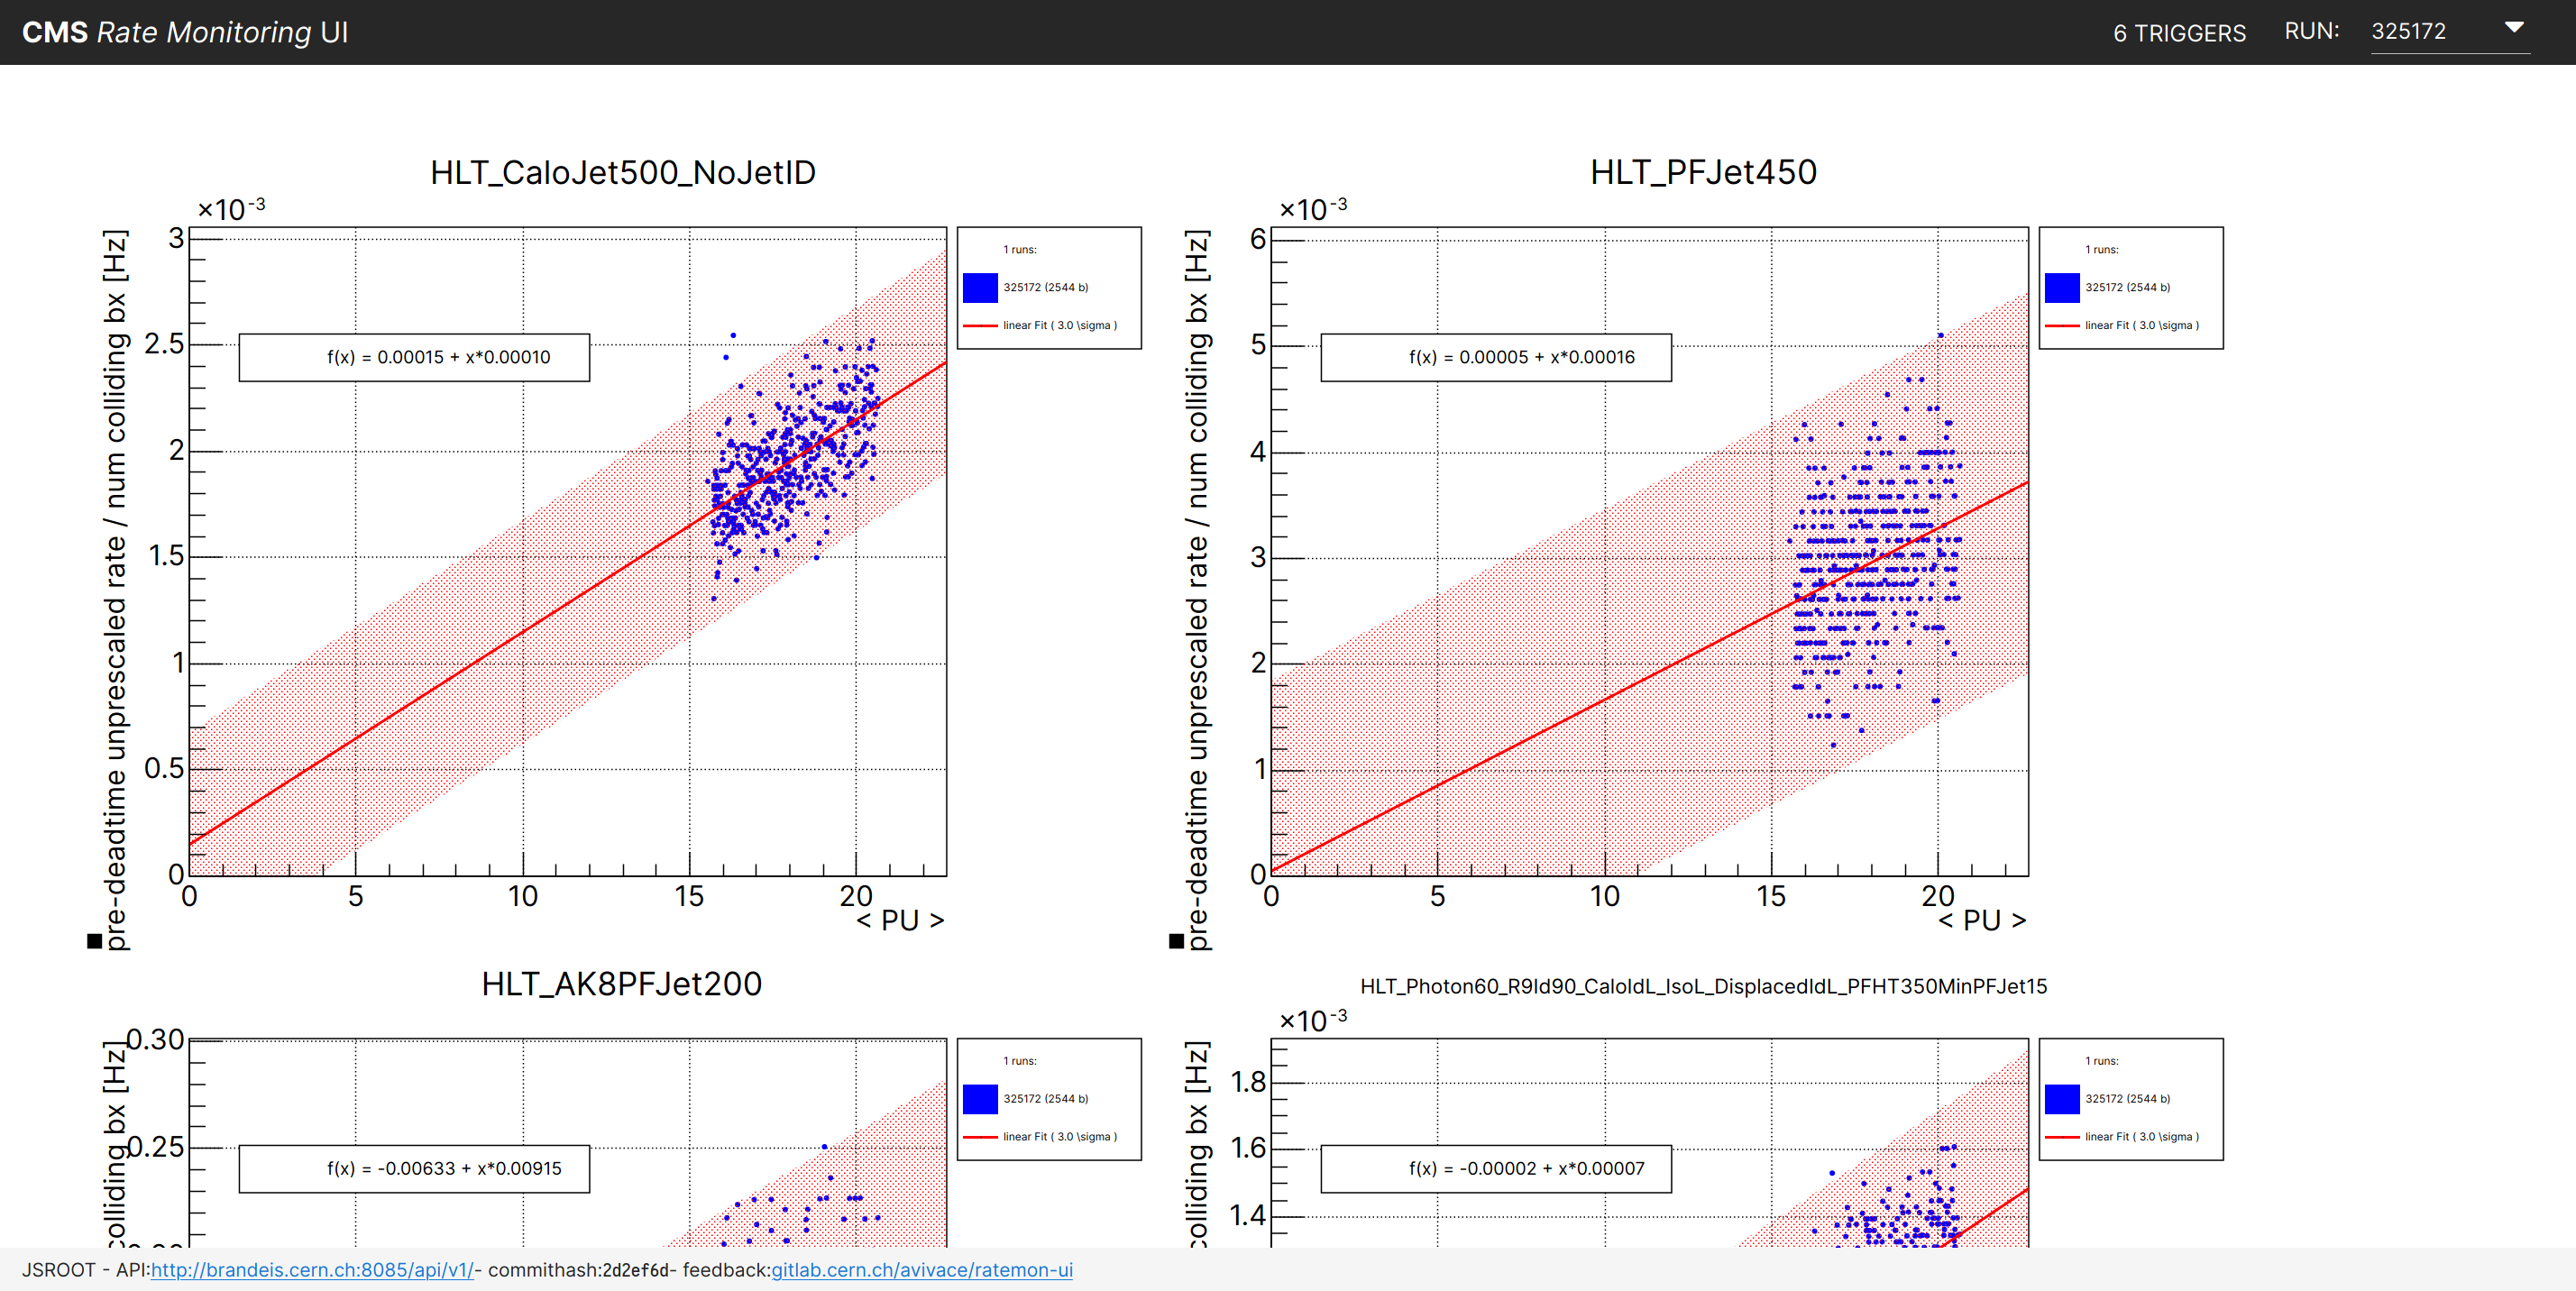
\includegraphics[width=0.9\paperwidth]{figures/ratemon-ui0.png}}
    \caption{Main RateMon UI application view, showing interactive trigger rate plots and relative fit functions}
    \label{fig:ratemon_ui0}
\end{figure}
 
\printbibliography
\thispagestyle{empty}

\end{document}